        \documentclass{article}
        \usepackage[margin=1in]{geometry}
        \usepackage{hyperref}
        \usepackage{amsmath,amsfonts,amssymb,amsthm,commath,dsfont}
        \usepackage{enumitem}
        \usepackage{bbold}
        \usepackage{amsmath}
        \usepackage{framed}
        \usepackage{xspace}
        \usepackage{booktabs}
        \usepackage{microtype}
        \usepackage{float}
        \usepackage[round]{natbib}
        \usepackage{cleveref}
        \usepackage[dvipsnames]{xcolor}
        \usepackage{graphicx}
        \usepackage{listings}
        \usepackage[breakable]{tcolorbox}
        \tcbset{breakable}
        \usepackage{bbm}
        \usepackage{mathtools}
        %\usepackage{symbols}
        \usepackage{subcaption}
        \usepackage{algorithm}
	\usepackage{algorithmic}

        
        \usepackage{pifont}
        \newcommand{\cmark}{\ding{51}}
        \newcommand{\xmark}{\ding{55}}
        \newcommand{\vect}[1]{\boldsymbol{#1}}
        \newcommand{\colbar}{\rule[-3mm]{.3mm}{1.5em}}
        \newcommand{\rowbar}{\rule[.5ex]{1.5em}{.3mm}}
        \DeclareMathOperator{\rank}{rank}
        \DeclareMathOperator*{\argmax}{argmax}
        \DeclareMathOperator*{\argmin}{argmin}

        % following loops stolen from djhsu
        \def\ddefloop#1{\ifx\ddefloop#1\else\ddef{#1}\expandafter\ddefloop\fi}
        % \bbA, \bbB, ...
        \def\ddef#1{\expandafter\def\csname bb#1\endcsname{\ensuremath{\mathbb{#1}}}}
        \ddefloop ABCDEFGHIJKLMNOPQRSTUVWXYZ\ddefloop
        
        % \cA, \cB, ...
        \def\ddef#1{\expandafter\def\csname c#1\endcsname{\ensuremath{\mathcal{#1}}}}
        \ddefloop ABCDEFGHIJKLMNOPQRSTUVWXYZ\ddefloop
        
        % \vA, \vB, ..., \va, \vb, ...
        \def\ddef#1{\expandafter\def\csname v#1\endcsname{\ensuremath{\boldsymbol{#1}}}}
        \ddefloop ABCDEFGHIJKLMNOPQRSTUVWXYZabcdefghijklmnopqrstuvwxyz\ddefloop
        
        % \valpha, \vbeta, ...,  \vGamma, \vDelta, ...,
        \def\ddef#1{\expandafter\def\csname v#1\endcsname{\ensuremath{\boldsymbol{\csname #1\endcsname}}}}
        \ddefloop {alpha}{beta}{gamma}{delta}{epsilon}{varepsilon}{zeta}{eta}{theta}{vartheta}{iota}{kappa}{lambda}{mu}{nu}{xi}{pi}{varpi}{rho}{varrho}{sigma}{varsigma}{tau}{upsilon}{phi}{varphi}{chi}{psi}{omega}{Gamma}{Delta}{Theta}{Lambda}{Xi}{Pi}{Sigma}{varSigma}{Upsilon}{Phi}{Psi}{Omega}{ell}\ddefloop

        \newcommand\T{{\scriptscriptstyle\mathsf{T}}}
        \def\diag{\textup{diag}}
        
      

        \def\SPAN{\textup{span}}
        \def\tu{\textup{u}}
        \def\R{\mathbb{R}}
        \def\E{\mathbb{E}}
        \def\Z{\mathbb{Z}}
        \def\be{\mathbf{e}}
        \def\nf{\nabla f}
        \def\veps{\varepsilon}
        \def\cl{\textup{cl}}
        \def\inte{\textup{int}}
        \def\dom{\textup{dom}}
        \def\Rad{\textup{Rad}}
        \def\lsq{\ell_{\textup{sq}}}
        \def\hcR{\widehat{\cR}}
        \def\hcRl{\hcR_\ell}
        \def\cRl{\cR_\ell}
        \def\hcE{\widehat{\cE}}
        \def\cEl{\cE_\ell}
        \def\hcEl{\hcE_\ell}
        \def\eps{\epsilon}
        \def\1{\mathds{1}}
        \newcommand{\red}[1]{{\color{red} #1}}
        \newcommand{\blue}[1]{{\color{blue} #1}}
        \def\srelu{\sigma_{\textup{r}}}
        \def\vsrelu{\vec{\sigma_{\textup{r}}}}
        \def\vol{\textup{vol}}

        \newcommand{\ip}[2]{\left\langle #1, #2 \right \rangle}
        \newcommand{\mjt}[1]{{\color{blue}\emph\textbf{[M:}~#1~\textbf{]}}}
        \newcommand{\sahand}[1]{{\color{green}\emph\textbf{[Sah:}~#1~\textbf{]}}}
		
        \newtheorem{fact}{Fact}
        \newtheorem{lemma}{Lemma}
        \newtheorem{condition}{Condition}
        \theoremstyle{definition}
        \theoremstyle{remark}
        \newtheorem{remark}{Remark}
        \newtheorem{example}{Example}

        \newenvironment{Q}
        {%
          \clearpage
          \item
        }

        \title{CS 446 / ECE 449 --- Homework 1}
        \author{\emph{acard6}}
        \date{Version 1.0}

        \begin{document}
        \maketitle

        \noindent\textbf{Instructions.}
        \begin{itemize}
          \item
            Homework is due \textbf{Tuesday, Feb 7th, at noon CDT}.
        
          \item
            Everyone must submit individually at gradescope under \texttt{hw1} and \texttt{hw1code}.
        
          \item
            The ``written'' submission at \texttt{hw1} \textbf{must be typed}, and submitted in
            any format gradescope accepts (to be safe, submit a PDF).  You may use \LaTeX, markdown,
            google docs, MS word, whatever you like; but it must be typed!
        
          \item
            When submitting at \texttt{hw1}, gradescope will ask you to mark out boxes
            around each of your answers; please do this precisely!
        
          \item
            Please make sure your NetID is clear and large on the first page of the homework.
        
          \item
            Your solution \textbf{must} be written in your own words.
            Please see the course webpage for full academic integrity information.
            Briefly, you may have high-level discussions with at most 3 classmates,
            whose NetIDs you should place on the first page of your solutions,
            and you should cite any external reference you use; despite all this,
            your solution must be written in your own words.
        
          \item
            We reserve the right to reduce the auto-graded score for
            \texttt{hw1code} if we detect funny business (e.g., your solution
            lacks any algorithm and hard-codes answers you obtained from
            someone else, or simply via trial-and-error with the autograder).
            
          \item
           When submitting to \texttt{hw1code}, only upload \texttt{hw1.py} and \texttt{hw1\_utils.py}. Additional files will be ignored.
        
        \end{itemize}
        \noindent\textbf{Version History.}
        \begin{enumerate}[leftmargin=3\parindent]
        	\item[1.0]
        	Initial Version. 
	\end{enumerate}
       
       \begin{enumerate}[font={\Large\bfseries},left=0pt]
	   \begin{Q}
\textbf{\Large Principal Component Analysis}\\

\begin{enumerate}

\item For each of the following statements, specify whether the statement is true or false. If you think the statement is wrong, explain in 1 to 2 sentences why it is wrong.


\begin{itemize}
\item True or False: As shown in the figure below, PCA seeks a subspace such that the sum of all the vertical distance to the subspace (the dashed line) is minimized.
\begin{center}
 \includegraphics[width=8cm]{figs/pca.pdf}
 \end{center}
\underline{\textbf{True}}


\item True or False: PCA seeks a projection that best represents the data in a least-squares sense.\\
\textbf{\underline{True}}

\item  True or False: PCA seeks a linear combination of variables such that the maximum variance is extracted from the variables.\\
\textbf{\underline{True}}

\item True or False: The principal components are not necessarily orthogonal to each other. \\
\textbf{\underline{False:}} PCA uses covariance matrix which are always symmetric and always have eigenvalues and vectors. The eigenvectors are always orthogonal to the symmetric matrix from which they stem from.

\end{itemize}


\item Recall that PCA finds a direction $w$ in which the projected data has highest variance by solving the following program:
	\begin{equation}
	\max_{w:||w||^2=1}w^T\Sigma w.
	\label{equ:pca}
	\end{equation}
	Here, $\Sigma$ is a covariance matrix. You are given a dataset of two 2-dimensional points $(1,3)$ and $(4,7)$. Draw the two data points on the 2D plane. What is the first principal component $w$ of this dataset?\\

$\mu_{x} = \frac{1+4}{2}=2.5, \mu_{y} = \frac{3+3}{2}=5$,  Cov(x,y) = $\sum^{2}_{i=1} \frac{(x_{i}-\mu_{x})*(y_{i}-\mu_{y})}{2} = 3$, Var(x)=2.25, Var(y)=4\\
$\Sigma = \left[ \begin{matrix}
2.25 & 3\\ 3 & 4 \end{matrix} \right]$\\
Its eigenvalues are $\lambda = 0, \frac{25}{4}$, our largest eigenvalue greater than 0 and its corresponding eigenvector is 
$\left[ \begin{matrix} 2.25 & 3\\ 3 & 4 \end{matrix} \right]\text{x} = \lambda\text{x} \rightarrow \left[ \begin{matrix} -3\\ 4 \end{matrix} \right]$.
\\


\item Now you are given a dataset of four points $(2,0)$, $(2,2)$, $(6,0)$ and $(6,2)$. Draw the four data points on the 2D plane. Given this dataset, what is the dimension of the covariance matrix $\Sigma$ in Eq.~\eqref{equ:pca}? Also, explicitly write down the values of $\Sigma$ given the dataset.

the mean and variance of x and y are $\mu_x = 4, \mu_y = 1, Var(x) = 4, Var(y) = 1,with the Cov(x,y) = 0$. The dimensions of the covariance matrix $\Sigma$ is 2, $$\Sigma = \left[\begin{matrix} 4 & 0 \\ 0 & 1\end{matrix} \right]$$

\item What is the optimal $w$ and the optimal value of the program in Eq.~\eqref{equ:pca}  given \[ \Sigma= \left[ \begin{array}{cccc}
	12 & 0 & 0 & 0\\
	0 & 6 & 0 & 0\\
	0 & 0 & 20 & 0\\
	0 & 0 & 0 & 10\\
	\end{array} \right].\] 
	
Knowing the optimal $w$ is found by taking the eigenvector of the largest eigenvalue of the covariance matrix, which after being computed leaves the eigenvalues to be $\lambda = 10, 12, 6, 20$, taking the largest value and finding its vector is is $\lambda = 20 \rightarrow \left[ \begin{matrix} 0 \\ 0 \\ 1 \\ 0 \end{matrix} \right]$ and plugginh this back into Eq. 1 we get $\max_{w:||w||^2=1}w^T\Sigma w = 20$


\end{enumerate}
\end{Q}
                   
    
    	 \begin{Q}
\textbf{\Large K-Means 1}\\

\begin{enumerate}

\item Mention if K-Means is a supervised or an un-supervised method and state the reason.\\
\textbf{Asnwer\: un-supervised}, since with kmean there is no requirement to label data of anysort, rather the algorithm is rather simply just clustering data together and dealing with distortion.

\item Assume that you are trying to cluster data points $x_{i}$  for $ i \in \{1,2, \dots, D\}$ into $K$ clusters each with center $\mu_{k}$  where $ k \in \{1,2, \dots, K \}$. The objective function for doing this clustering involves minimization of the Euclidean distance between the points and the cluster centers. It is given by  \begin{equation*}
\min\limits_{\mu} \min\limits_{r}\sum\limits_{i \in D} \sum\limits_{k =1}^{K} \frac{1}{2} r_{ik} \|x_{i} -\mu_{k}\|_{2}^{2}. \\
 \end{equation*} \\ How do you ensure hard assignment of one data point to one and only one cluster at a given time?
 
 \textbf{Hint:} By hard assignment we mean that you are 100 \% sure that a point either belongs or doesn't belong to a cluster.\\
\textbf{Answer:} to best ensure that we are 100\% certain about what cluster a point belongs to we look to see what cluster minimizes its distance to the point and if it just so happens that a point is equdistance from multiple cluster then we simply just take the first cluster presented
 
 \item How does your answer to part b change if we want to obtain a soft assignment instead?
 
 \textbf{Hint:} By soft assignment we mean that  a point  belongs to a cluster with some probability.\\
\textbf{Answer:}If we were to use soft clustering then we could use percentages and probability where a point would stores a the likelihood that its near a certain cluster since we no longer have to worry about beign set to one main cluster, but rather the likelyhood of being in a cluster. This leaves us with less ambiguity as to what to do with points that have clusters with equal probability since they can belong to multiple.
 
 \item Looking at the following plot, what is the best choice for the number of clusters?
 \begin{center}
 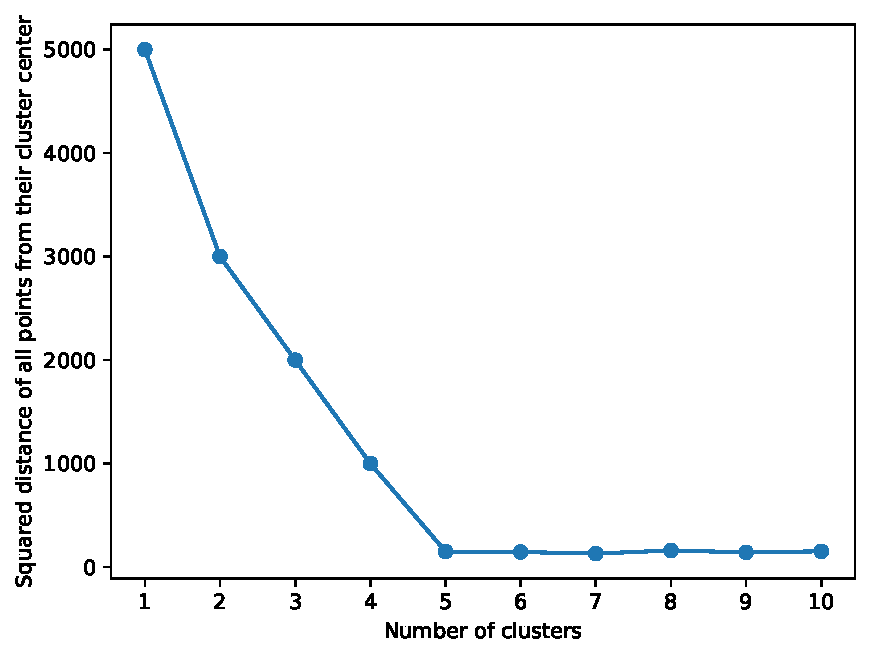
\includegraphics[width=8cm]{figs/cluster.pdf}
 \end{center}
 \textbf{Answer:} since after 5 clusters and onward the spread from the cluster center seems to level out the best choice is 5 clusters.
 
 \item Would K-Means be an efficient algorithm to cluster the following data? Explain your answer in a couple of lines.
 \begin{center}
 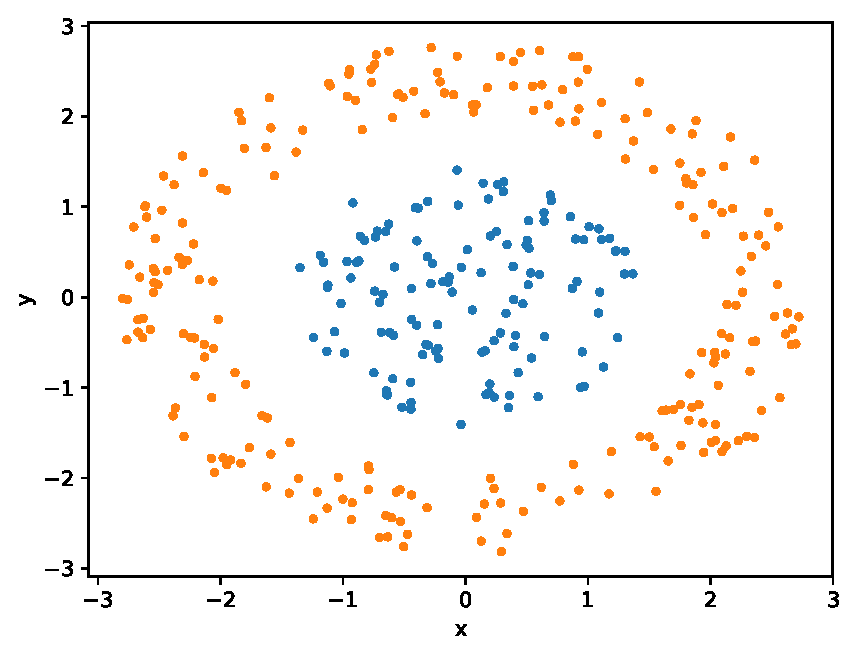
\includegraphics[width=8cm]{figs/concentric.pdf}
 \end{center}
 \textbf{Answer:} No, since trying to classify the data into two distinct groups would require multiple groups. The overall mean of all the datapoints is the center of the and trying to tether the outter ring to a single cluster would be hard for that reason it is unreasonable to use k-mean clustering for this data

\end{enumerate}


\end{Q}
                      
	  
	  \begin{Q}
\textbf{\Large K-Means 2}\\

We are given a dataset $\cD = \{(x)\}$ of 2d points $x\in\mathbb{R}^2$ which we are interested in partitioning into $K$ clusters, each having a cluster center $\mu_k$ ($k\in\{1, \ldots, K\}$) via the $k$-Means algorithm. This algorithm optimizes the following cost function:
\begin{equation}
	\min_{\mu_k, r} \sum_{x\in\cD,k\in\{1, \ldots, K\}} \frac{1}{2}r_{x,k}\|x - \mu_k\|_2^2 \quad\quad\text{s.t.}\quad \left\{\begin{array}{ll}
r_{x,k}\in\{0,1\}&\forall x\in\cD,k\in\{1, \ldots, K\}\\
\sum_{k\in\{1, \ldots, K\}} r_{x,k} = 1 & \forall x\in\cD
\end{array}\right.
\label{eq:KMeans2:main}
\end{equation}

\begin{enumerate}

\item What is the domain for $\mu_k$?

\item Given fixed cluster centers $\mu_k$ $\forall k\in\{1, \ldots, K\}$, what is the optimal $r_{x,k}$ for the program in Eq. \ref{eq:KMeans2:main}? Provide a reason?

\item Given fixed $r_{x,k}$ $\forall x\in\cD,k\in\{1, \ldots, K\}$, what are the optimal cluster centers $\mu_k$ $\forall k\in\{1, \ldots, K\}$ for the program in Eq. \ref{eq:KMeans2:main}? 

\textbf{Hint:} Reason by first computing the derivative w.r.t $\mu_k$.

\item Using Pseudo-code, sketch the algorithm which alternates the aforementioned two steps. Is this algorithm guaranteed to converge and why? Is this algorithm guaranteed to find the global optimum? What is the reason?

\textbf{Hint:} you can provide a counter-example to invalidate a statement.

\item Please implement the aforementioned two steps. For the given dataset, after how many updates does the algorithm converge, what cost function value does it converge to and what are the obtained cluster centers? Visualize clusters at each step and attach the plots here. Please at least report numbers with one decimal point.

\textbf{Remark:} how we count updates: when computing a set of new centroids from initialization, we call this one update.

\textbf{Hint:} You may find \texttt{hw1\_utils.vis\_cluster} useful.

\end{enumerate}

%%%%%%%%%%%%%%%%%%  ANSWERS  %%%%%%%%%%%%%%%%
\begin{itemize}
\item[\textit{Answer A)}] If the data is in the 2D-plane then the domain of $\mu_k$ is also 2D as a real value
\item[\textit{Answer B)}] The optimal $r_{x,k}$  is   \begin{equation} r_{x,k} = \begin{cases} 1 & \text{for} \arg \min_{k} |x^{i} - \mu_k |^2 \\ 0 & \text{else} \end{cases} \end{equation}
\item[\textit{Answer C)}] The optimal cluster centers $\mu_k \forall$ is $$\mu_k = \frac{\sum_{i \in D} r_{ik} x^{(i)}}{\sum_{i \in D} r_{ik}}$$
\item[\textit{Answer D)}]  The following algorithm may not always be guaranteed to find global optimal since there is a possibility that when initializing the random starting centroids it can get stuck in local minima and not reach the correct optimum. To overcome this issue it is best to run it many times with different initial cluster centroid to ensure that optimum can be found.\\
\begin{algorithm} 
\caption{k-means clustering} 
\begin{algorithmic} 
\STATE Input $\mathcal{D} \leftarrow$ set of 2D points
\STATE Input K $\leftarrow$ number of cluster centroid $\mu_k$
\STATE randomly assign centroids to points in data
\REPEAT
\FOR {iteration $\leftarrow$ 1 to max\_iter}
\FORALL {$x_i \in \mathcal{D}$}
\STATE $r_{ik} \leftarrow \arg \min_k ||x_i-\mu_k||^2$
\ENDFOR
\FOR {$k \leftarrow 1 to K$}
\STATE $\mu_k \leftarrow (\sum x^i $ that are a part of that $\mu_k$) / (the number of points in the $\mu_k$) 
\ENDFOR
\ENDFOR
\UNTIL {max iteration or all cluster $\mu_k$ reach equalibrium}
\end{algorithmic} 
\end{algorithm}


% \STATE to say something
% \IF{<condition>} <text> \ELSIF{<condition>} <text> \ELSE <text> \ENDIF
% \WHILE{<condition>} <text> \ENDWHILE
% \LOOP <text> \ENDLOOP
% \FOR{<condition>} <text> \ENDFOR


\end{itemize}


\end{Q}
                    
       
        \begin{Q}
\textbf{\Large Gaussian Mixture Models}\\

Consider a Gaussian mixture model with $K$ components ($k\in\{1, \ldots, K\}$), each having mean $\mu_k$, variance $\sigma_k^2$, and mixture weight $\pi_k$. Further, we are given a dataset $\mathcal{D} = \{x_i\}$, where $x_i \in \mathbb{R}$. We use $z_{i} = \{z_{ik}\}$ to denote the latent variables.


\begin{enumerate}

\item What is the log-likelihood of the data according to the Gaussian Mixture Model (use $\mu_k$, $\sigma_k$, $\pi_k$, $K$, $x_i$, and $\mathcal{D}$)?

\item Assume $K=1$,  find the maximum likelihood estimate for the parameters ($\mu_{1}$, $\sigma_{1}^{2}$, $\pi_{1}$).

\item What is the probability distribution on the latent variables, i.e., what is the distribution
$p(z_{i,1}, z_{i,2}, \cdots, z_{i,K} )$ underlying Gaussian mixture models. Also give its name.


\item For general $K$, what is the posterior probability $p(z_{ik} = 1|x_i)$? To simplify, wherever possible, use $\mathcal{N}(x_{i}|\mu_{k},\sigma_{k})$, a Gaussian distribution over $x_{i} \in \mathbb{R}$ having mean $\mu_{k}$ and variance $\sigma_{k}^2$.


\item  How are k-Means and Gaussian Mixture Model related? (There are three conditions)

\textbf{Hint:} Think of variance, $\pi_k$, and hard/soft assignment.

\item  Show that:
$$
\lim_{\epsilon \rightarrow 0} -\epsilon \log \sum_{k=1}^{K} \exp{(-F_{k}/\epsilon) } = \min_{k} F_{k}, \quad \epsilon \in \mathbb{R}^{+}
$$
\textbf{Hint:} Use l'Hopital's rule.

\item Consider the modified Gaussian Mixture Model objective:
$$
\min_{\mu} - \sum_{x_{i} \in \mathcal{D}} \epsilon \log \sum_{k=1}^{K} \exp{(-(x_{i} - \mu_{k} )^{2}/\epsilon) }.
$$
Conclude that the objective for k-Means is the 0-temperature limit of Gaussian Mixture Model.

\textbf{Hint:} Let $F_{k}= (x-\mu_{k})^{2}$ and apply the equation you proved in (f).

\end{enumerate}

\begin{itemize}
\item[\textit{Answer A)}] The log likelihood of of $p(x_i |\pi, \mu, \sigma) = \sum_{k=1}^K \pi_k \mathcal{N}(x^{(i)}|\mu_k,\sigma_k)$ is $log(\sum_{k=1}^K \pi_k \mathcal{N}(x_i|\mu_k,\sigma_k) )$

\item[\textit{Answer B)}] Assuming that $K = 1$ we can find the MLE by maximizing the log-likelihood function, which in this case is $log(N(x_i|\mu_k,\sigma_k)= log(p(x_i)|\mu, \sigma) = \sum_(i \in \mathcal{D}) \frac{(x_i-\mu)^2}{2 \sigma^2}+ \frac{N}{2}log(2\pi \sigma^2) $, where N is the size of the dataset. since K=1 there is no need for summation and $\pi_1=1$ since it can be no other value. Thus maximizing the MLE for $\mu$ and $\sigma$, we get the sample mean and variance $\mu = \frac{1}{N}\sum_{i \in \mathcal{D}}x_i  \text{,   }\sigma^2 = \frac{1}{N}\sum_{i \in \mathcal{D}}(x_i-\mu)^2$

\item[\textit{Answer C)}] the probability of the auxiliary variable is $p(z_{ik}=1) =\pi_k \text{, } \Pi^K_{k=1}\pi_k^{z_{ik}},  z_i= [z_{i1},\text{...},z_{iK}]^T$

\item[\textit{Answer D)}] for a general K the posterior probability is $p(z_{ik}|x_i) = \frac{\pi_k \mathcal{N}(x_i|\mu_k,\sigma_k)}{\sum^K_{\widehat{k}=1} \pi_{\widehat{k}} \mathcal{N}(x_i|\mu_{\widehat{k}},\sigma_{\widehat{k}})}$

\item[\textit{Answer E)}] while both kmean and gmm are unsupervised learning techniques that use pre-determined clusters numbers, they relate in how they label the datas relation to one another using distance to determine how related they are to the rest of the data in some shape. As well as their use of the variance of the data to better form relations between each iteration to better fit a mold for the data, and determing how to assign data to a cluster whether the use of probability $\pi$ or not.

\item[\textit{Answer F)}] so consider $f(\epsilon) = -epsilon, g(\epsilon) = \sum_{k=1}^K exp(-F_k/\epsilon), h(\epsilon) = log(g(\epsilon))$ the limit as f approaches 0 is 0 and the limit as h approaches 0 from the right is $log \sum_{k=1}^K exp(-F_k/\epsilon) = log \sum_{k=1}^K exp(-\inf) = log(k*0) = log(0) \rightarrow \lim_{x\rightarrow 0^+} log(x) = -\inf$ so we get $\lim_{\epsilon \rightarrow 0} f(\epsilon)h(\epsilon)=0*-\inf$ by l'Hopitals we get $f'(\epsilon) = -1, h'(\epsilon) = \frac{1}{g(\epsilon)}g'(\epsilon) = \frac{\sum_{k=1}^k F_k*exp(-F_k/\epsilon)}{\epsilon^2 \sum_{k=1}^K exp(-F_k/\epsilon)} = \frac{1}{\epsilon^2} \sum_{k=1}^K \frac{F_k*exp(-F_k/\epsilon)}{exp(-F_k/\epsilon)} = \sum \frac{F_k}{\epsilon^2}$
$$\lim_{\epsilon \rightarrow 0} \sum_{k=1}^K F_k/\epsilon^2 = \lim_{\epsilon \rightarrow 0} \frac{d^2}{d\epsilon^2} \sum^K_{k=1} F_k/\epsilon^2 = \min_{k} F_k / 1 = \min_k F_k$$

\item[\textit{Answer G)}] if $F_k = (x-\mu_k)^2$ then $$\lim_{\epsilon \rightarrow 0^+} \min_{\mu} -\sum_{x_i \in \mathcal(D)} \epsilon log \sum exp(F_k/\epsilon) = \min_{\mu} \sum_{x_i \in \mathcal(D)}  min_{k} F_k = \min_{\mu} \min_k \sum_{x_i \in \mathcal{D}} (x_i - \mu)^2$$ is the cost function of k-means clustering, therefore the k-mean is the 0-temp limit of the gaussian mixture model
 
\end{itemize}


\end{Q}
          
        
	 
 
    \end{enumerate}
    
    \textbf{Appendix}
     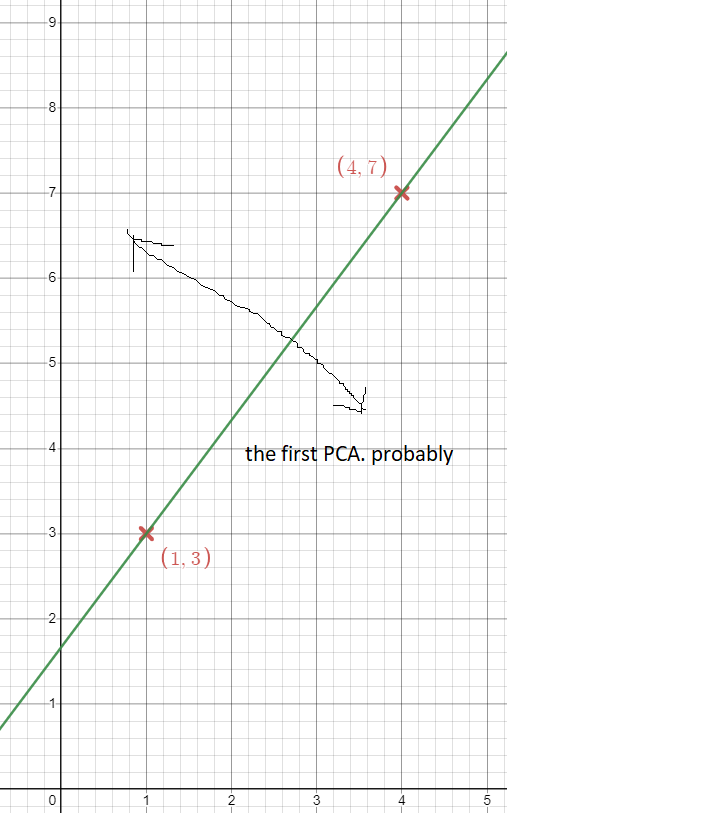
\includegraphics[scale=0.5]{figs/pca1.png}\\
     \textbf{figure 1:} the drawing for Q1 part b\\
     
     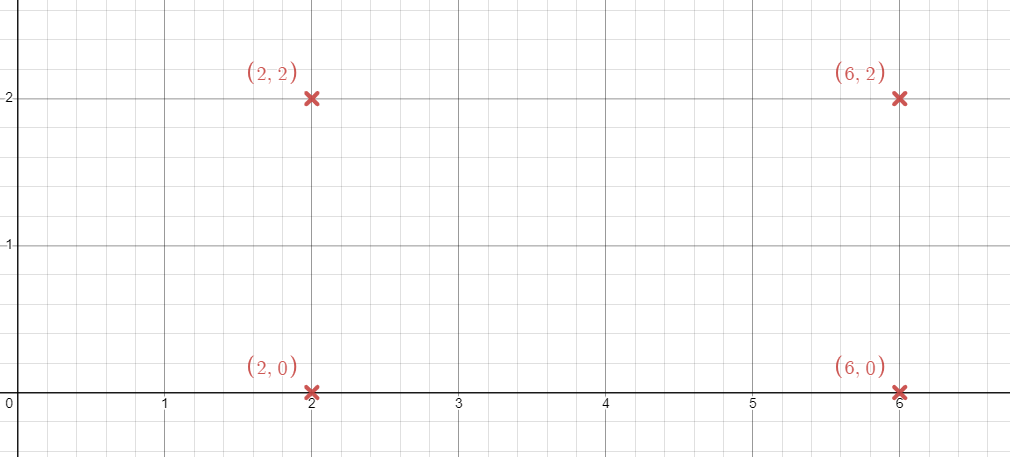
\includegraphics[scale=0.5]{figs/pca2.png}\\
     \textbf{figure 2:} the drawing for Q1 part c
\end{document}
